% 1 kolonne
\documentclass[aps,rmp,preprint,amsmath,amssymb,longbibliography,floatfix]{revtex4-1}

% 2 kolonner
%\documentclass[aps,rmp,reprint,amsmath,amssymb,longbibliography,twocolumn,floatfix]{revtex4-1}

% Include the configuration file
\usepackage{bm}
\usepackage{graphicx}
\usepackage{epstopdf}
\usepackage{wrapfig}
\usepackage{array} 
\usepackage{listings}
\usepackage[para,online,flushleft]{threeparttablex}
% \usepackage{booktabs,dcolumn}
\usepackage{color}
\usepackage{comment}

\usepackage{tcolorbox}  % For better styled boxes
 
\usepackage{textpos}
% \usepackage{booktabs}
\usepackage{multirow,bigdelim}
\usepackage{tikz}
\usepackage{dsfont}
% \usepackage{subfigure}
\usepackage{float}
% \usepackage{caption}
% \usepackage{subcaption}
\usepackage{subfig}
\usepackage{pgfplots}
\usepackage{microtype}
% \usepackage{tabularx}

\pgfplotsset{width=\textwidth*0.5, height=\textwidth/3*0.5,compat=1.18}

\usepackage[super]{nth}

\usepackage{upgreek} %upalpha in Saxena2021 Reference

\usepackage[utf8]{inputenc}
\usepackage{hyperref}
\hypersetup{breaklinks=true,colorlinks=true,linkcolor=blue,citecolor=blue,filecolor=magenta,urlcolor=blue}

\usepackage{lipsum}


\usepackage{xcolor}
%\newcommand{\contrib}[1]{\textcolor{red}{#1}}
%\newcommand{\comment}[1]{\textcolor{blue}{#1}}

%\newcommand{\WN}[1]{{\color{red} #1}}

\makeatletter
\def\@bibdataout@aps{%
\immediate\write\@bibdataout{%
@CONTROL{%
apsrev41Control%
\longbibliography@sw{%
    ,author="08",editor="1",pages="1",title="0",year="1"%
    }{%
    ,author="08",editor="1",pages="1",title="",year="1"%
    }%
  }%
}%
\if@filesw \immediate \write \@auxout {\string \citation {apsrev41Control}}\fi
}
\makeatother

\DeclareMathOperator*{\argmax}{arg\,max}
\DeclareMathOperator*{\argmin}{arg\,min}
\DeclareMathOperator{\MSE}{MSE}
\DeclareMathOperator*{\compfunc}{\bigcirc}

\newcommand{\mia}[1]{\textbf{\textcolor{magenta}{#1}}}
\newcommand{\jonatan}[1]{\textbf{\textcolor{blue}{#1}}}
\newcommand{\benjamin}[1]{\textbf{\textcolor{green
}{#1}}}

% Shortcuts
\newcommand{\g}{\mathbf{g}}


% \bibliographystyle{apsrev4-1}
%\usepackage[left]{lineno}
%\linenumbers

\begin{document}

\title{Working title: Project 1 FYS4150}

\author{Merlid, Winsvold and Gressløs}
% \affiliation{Department of Mathematics, University of Oslo, N-0316 Oslo, Norway}
\date{\today}
\affiliation{University of Oslo}


\begin{abstract}
\input{project_1/text/0_abstract}
\end{abstract}

\maketitle

\tableofcontents

\section*{Problem 1}


The one-dimensional Poisson equation can be written as:

\begin{equation}
   -\frac{du^2(x)}{dx^2} = f(x)
    \label{poisson_eq} 
\end{equation}


Will check analytically if $u(x) = 1 - (1 - e^{-10}) x - e^{-10x} $ is a solution to Eq. \ref{poisson_eq} for a given source term $f(x) = 100e^{-10x}$. The expression also fulfills the Dirichlet boundary conditions $u(0) = u(1) = 0$.


\begin{align}
    -\frac{du^2(x)}{dx^2} &= -\frac{d}{dx}(-1 + e^{-10} + 10e^{-10x}) \\
    &= 100e^{-10x} \\
    &= \underline{\underline{f(x)}}
\end{align}\label{sec:prob1}


\section*{Problem 2}
Plotting the solution to the one-dimensional Poisson equation, \(u(x)\), described in Problem 1 in Fig. \ref{fig:task2_plot}.

\begin{figure}
    \centering
    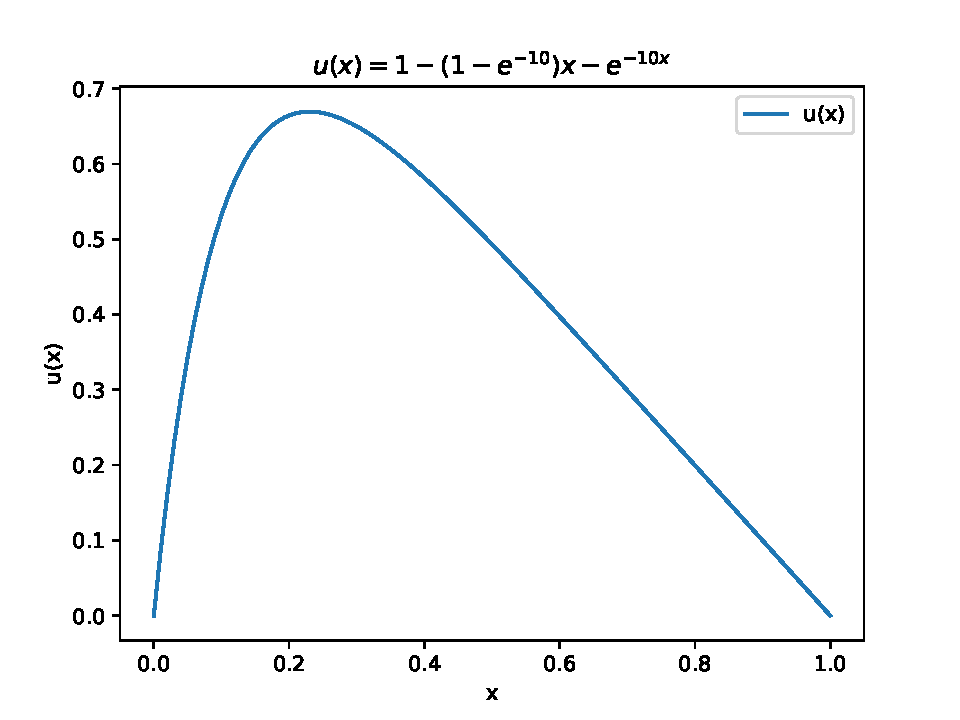
\includegraphics[width=0.5\linewidth]{project_1/text/plot_t2.pdf}
    \caption{Plot for Problem 2}
    \label{fig:task2_plot}
\end{figure}\label{sec:prob2}


\section*{Problem 3}
The discretized version of the Poisson equation expressed using the double derivative approximation:
\begin{align}
    \frac{d^2u}{dx^2}  &= \frac{u_{i+1} - 2u_{i} + u_{i-1}}{(\Delta x)^2} + O(\Delta x^2)  \\
    \frac{d^2u}{dx^2} &\sim \frac{v_{i+1} - 2v_{i} + v_{i-1}}{(\Delta x)^2}
    \label{derivative_approx}
\end{align}

Define $v_i$ as the discretized approximation to $u_i$. The result in Eq. \ref{derivative_approx} is derived from adding the Taylor Expansion for $x_{i+1} $ and $x_{i-1}$ around point $x_i$ for $\Delta x^2 = h$: 
\begin{align*}
    u_{i+1} = u_i + u'h + \frac{1}{2}u''^2 + \frac{1}{6}u'''h^3 + O(h^4)\\
    u_{i-1} = u_i - u'h + \frac{1}{2}u''h^2 - \frac{1}{6}u'''h^3 + O(h^4) 
\end{align*}

The elimination of odd powers explane the order of error $O(\Delta x^2)$. Combining Eq. \ref{poisson_eq} and \ref{derivative_approx} gives:
\begin{align}
    v_{i+1} - 2v_{i} + v_{i-1} = (\Delta x)^2 f(x)
\end{align}


\label{sec:prob3}


\section*{Problem 4}

If we denote the vector of unknowns in Eq. \ref{discretization} as \( \mathbf{v} = [v_1, v_2, \ldots, v_n]^T \), the system of equations can be represented in matrix form as:


\begin{align}
    A \mathbf{v} = \mathbf{g}
    \label{Avg}
\end{align}

where
$$
    \g = \begin{pmatrix}
(\Delta x)^2 f_1 + v_0 \\
(\Delta x)^2 f_2 \\
(\Delta x)^2 f_3 \\
\vdots \\
(\Delta x)^2 f_{n-1} \\
(\Delta x)^2 f_n + v_{n+1}
\end{pmatrix}

$$

%\( \mathbf{g} = \frac{100}{n^2} [e^{\frac{-10}{n}}, e^{\frac{-20}{n}}, \ldots, e^{-10}]^T \) 


and \( \mathbf{A} \) is an \(n \times n\) tridiagonal matrix of the form:

\[
\mathbf{A} = \begin{pmatrix}
2 & -1 & 0 & \cdots & 0 \\
-1 & 2 & -1 & \cdots & 0 \\
0 & -1 & 2 & \cdots & 0 \\
\vdots & \vdots & \vdots & \ddots & \vdots \\
0 & 0 & 0 & \cdots & 2
\end{pmatrix}
\]

This matrix \( \mathbf{A} \) has the subdiagonal, main diagonal, and superdiagonal specified by the signature \( (-1, 2, -1) \). Specifically, the elements of \( \mathbf{A} \) are related to the coefficients in the discretized Eq. \ref{discretization} as follows:

- The main diagonal elements \( A_{ii} \) correspond to the coefficient of \( b_i \), which is \( 2 \).

- The subdiagonal elements \( A_{i,i-1} \) and the superdiagonal elements \( A_{i,i+1} \) correspond to the coefficients of \( a_{i} \) and \( c_{i} \), respectively, which are \( -1 \).

Therefore, the matrix equation for the discretized system is:

\[
\begin{pmatrix}
2 & -1 & 0 & \cdots & 0 \\
-1 & 2 & -1 & \cdots & 0 \\
0 & -1 & 2 & \cdots & 0 \\
\vdots & \vdots & \vdots & \ddots & \vdots \\
0 & 0 & 0 & \cdots & 2
\end{pmatrix}
\begin{pmatrix}
v_1 \\
v_2 \\
v_3 \\
\vdots \\
v_n
\end{pmatrix}
=
\begin{pmatrix}
g_1 \\
g_2 \\
g_3 \\
\vdots \\
g_n
\end{pmatrix}
\]

where the vector \( \mathbf{g} \) on the right-hand side represents the source terms modified by the grid spacing \( h^2 f_i \).\label{sec:prob4}

\section*{Problem 5}
\subsubsection{a)}

We know that $\mathbf{v}$ has length $n$ and A is of dimension $n\times n$. The complete solution $\mathbf{v}^*$ has two additional point compared to $\mathbf{v}$, namely the two endpoints $\mathbf{v}_0$ and $ \mathbf{v_{n+1}} $. The relation between m, the length of $\mathbf{v}^*$ and $\mathbf{v}$ is given by $m = n+2$. 

\subsubsection{b)}

When we solve Eq. \ref{Avg} for $\mathbf{v}$ we find $v_i$ for $i = 1,2, \cdots n$. The missing values compared to $\mathbf{v}^*$ are $\mathbf{v}_0$ and $\mathbf{v}_{n+1}$ which are already known. \label{sec:prob5}

\section*{Problem 6}
Will solve $\mathbf{A} \mathbf{v} = \mathbf{g}$ by the Thomas Algorithm, which is a specialiced form of Gaussian elimination,   given A is a tridiagonal matrix. The derivation of the Thomas Algorithm was reviewed in the Lecture 4 \cite{lecture_notes}. The algorithm is built up of forward and backward substitution explaned below:


\begin{tcolorbox}[colback=lightgray!20, colframe=black, title=Forward Substitution]
\[
\tilde{b}_1 = b_1
\]

\[
\tilde{b}_i = b_i - \frac{a_i}{\tilde{b}_{i-1}} c_{i-1} \quad i = 2, 3, ..., n
\]

\[
\tilde{g}_1 = g_1
\]

\[
\tilde{g}_i = g_i - \frac{a_i}{\tilde{b}_{i-1}} \tilde{g}_{i-1} \quad i = 2, 3, ..., n
\]
\end{tcolorbox}


\begin{tcolorbox}[colback=lightgray!20, colframe=black, title=Back Substitution]
\[
v_n = \frac{\tilde{g}_n}{\tilde{b}_n}
\]

\[
v_i = \frac{\tilde{g}_i - c_i v_{i+1}}{\tilde{b}_i} \quad i = n-1, ..., 2, 1
\]
\end{tcolorbox}



The signature (-1,2,-1) of the tridiagonal matrix A result in every $a_i, b_i, c_i$ takes the respective values of the signature, thus -1, 2 and -1. 


Before counting floating-point operations (FLOPs) for this algorithm, will note $\frac{a_i}{\tilde{b}_{i-1}}$ is being iterated over $(n-1)$ times in both steps in the forward substitution. Will define a value $w_i = \frac{a_i}{\tilde{b}_{i-1}}$ which will reduce FLOPs by $n-1$ calculations.

Numbers of FLOPs becomes $3(n-1) +  2(n-1) = 5 (n-1)$ FLOPs for the forward substitutions and $(n-1) + 3 (n-1)$ FLOPs for the backward substitutions. This result in a total of $9(n-1)$ FLOPs for the general algorithm.


\label{sec:prob6}

\section*{Problem 7}
The plot of the comparison of the exact solution $u(x)$ against the numeric solutions for different values of $n_{steps} = n - 1$, where n is numbers of points, is found in Fig. \ref{task7} 

\begin{figure}
    \centering
    \includegraphics[width=0.5\linewidth]{}
    \caption{With $n_{steps}$ being the number of discretization steps along the x axis.}
    \label{fig:task7}
\end{figure}
\label{sec:prob7}

\section*{Problem 8}
\subsubsection{a and b}

The plots of the logarithm of base 10 of the absolute- and relative error is found in Fig. \ref{task8ab}. 

\begin{figure}
    \centering
    \includegraphics[width=0.5\linewidth]{}
    \caption{Show the respective errors for different choices of $n_{steps}$. Since the two boundary points are fixed (u(0) and u(1)), those points are left out in this error analysis.}
    \label{fig:task8ab}
\end{figure}


\subsubsection{c}
Table    shows the maximum relative error $max(\epsilon_i)$ for each choice of $n_{steps}$. The plot is found in Fig. \ref{task8c} 

\begin{figure}
    \centering
    \includegraphics[width=0.5\linewidth]{}
    \caption{Maximum relative error $max(\epsilon_i)$ for each choice of $n_{steps}$}
    \label{fig:task8c}
\end{figure}

\label{sec:prob8}

\section*{Problem 9}

We know that $(a_i, b_i, c_i) = (-1,2,-1)$ for all $i$, hence 
$$
    \tilde{b}_i = b_i - \frac{a_i}{\tilde{b}_{i-1}} c_{i-1}
    = 2- \frac{1}{\tilde{b}_{i-1}}
$$
We claim that $\tilde{b}_n = \frac{n+1}{n}$
\\\\
Proof of claim:
As a base case we have that $\tilde{b}_1 = b_1 = \frac{2}{1}$
If we assume that $\tilde{b}_n = \frac{n+1}{n}$ then it follow that
\begin{align*}
    \tilde{b}_{n+1} &= 2- \frac{1}{\tilde{b}_{i-1}} \\
    &= \frac{2n+2}{n+1} - \frac{n}{n+1} \\
    &= \frac{n+2}{n+1}
\end{align*}
Hence by induction over $n$ we have shown that $\tilde{b}_n = \frac{n}{n+1}$

The complexity of $\tilde{b}_n = \frac{n}{n+1}$ is 2 flops (addition and division) and the complexity of $\tilde{b}_i = b_i - \frac{a_i}{\tilde{b}_{i-1}} c_{i-1}$ is 4 flops, hence the loop has been reduced from 3(n-1) to 2(n-1) flops.

The total FLOPs from the specilized algorithm is therefore reduced from $9(n-1)$ to  $8(n-1)$ calculations.

\label{sec:prob9}


%\section*{Introduction}
%\input{project_1/text/1_introduction}\label{sec:introduction}

%\section*{Theory}
%\input{project_1/text/2_theory}\label{sec:theory}

%\section*{Method}
%\input{project_1/text/3_method}\label{sec:method}

%\section*{Results}
%\input{project_1/text/4_results_discussion}\label{sec:results}

%\section*{Conclusion}
%\input{project_1/text/5_conclusion}\label{sec:conclusion}

\newpage
\bibliography{project_1/References} % add references to this file

\appendix
\input{project_1/text/6_appendix}

\end{document}
